\documentclass{VUMIFPSbakalaurinis}
\usepackage{float}
\usepackage{hyperref}
\usepackage{algorithmicx}
\usepackage{algorithm}
\usepackage{algpseudocode}
\usepackage{amsfonts}
\usepackage{amsmath}
\usepackage{bm}
\usepackage{caption}
\usepackage{color}
\usepackage{graphicx}
\usepackage{listings}
\usepackage{subcaption}
\usepackage{wrapfig}
\usepackage{biblatex}
\usepackage{microtype}
\usepackage{mathtools}
\usepackage{multirow}

% Titulinio aprašas
\university{Vilniaus universitetss}
\faculty{Matematikos ir informatikos fakultetas}
\institute{Informatikos institutas}  % Užkomentavus šią eilutę - institutas neįtraukiamas į titulinį
\department{Programų sistemų bakalauro studijų programa}
\papertype{Laboratorinio darbo ataskaita}
\title{Tiesioginio sklidimo DNT modeliavimas naudojant sistemą WEKA}
\titleineng{Feedforward Neural Network Model Creation in WEKA}
\author{Armintas Pakenis}
% \secondauthor{Vardonis Pavardonis}   % Pridėti antrą autorių
\supervisor{prof. dr. Olga Kurasova}
\reviewer{prof. dr. Olga Kurasova}
% \addsignatureplaces{} % prideda parašų vietas tituliniame puslapyje
\date{Vilnius – \the\year}

\bibliography{bibliografija}

\begin{document}
\maketitle

%% Padėkų skyrius
% \sectionnonumnocontent{}
% \vspace{7cm}
% \begin{center}
%     Padėkos asmenims ir/ar organizacijoms
% \end{center}

\tableofcontents

\section{Užduoties tikslas}
Užduoties tikslas — išmokyti neuroninį tinklą teisingai
klasifikuoti duomenis naudojant sistemą WEKA. 
Išsaugotus WEKA procesus ir gautus programos rezultatus
galima rasti GitHub repositorijoje: 
\href{https://github.com/ArmintasP/Computational-intelligence/tree/main/Lab3}{\color{cyan}{https://github.com/ArmintasP/Computational-intelligence/tree/main/Lab3}}.

\subsection{Duomenys}
Naudotas irisų duomenų rinkinys: 
\href{https://archive.ics.uci.edu/ml/datasets/iris}{\color{cyan}{https://archive.ics.uci.edu/ml/datasets/iris}}.

Irisų duomenų rinkinys buvo išskaidytas į du rinkinius.
Vieną rinkinį sudarė 120 įrašų jis buvo naudojamas modeliui mokyti ir validuoti,
tad jį naudojant buvo vykdoma kryžminė patikra.
Kitą rinkinį sudarė likę 30 įrašų (po 10 iš kiekvienos klasės), 
kuris buvo naudojamas tik modeliui validuoti.

\section{Užduočių sekų modeliavimas}

\ref{img:1-seka} paveikslėlyje matoma užduoties seka naudoja
120 įrašų duomenų rinkinį. \textit{ArffLoader} komponentas
užkrauna duomenų rinkinį, \textit{ClassAssigner} nustato,
kelinta įeitis bus laikoma klasės žyme. 
\textit{CrossValidation FoldMaker} suskaido duomenų rinkinį
į N poabių (darbe buvo naudojama 10 poaibių), kur N-1 poaibių
bus naudojama mokymui, o likęs vienas — validavimui.
\textit{Multilayer Perceptron} — neuroninis tinklas, iš kurio
rezultatai keliauja į \textit{Classifier Performance Evaluator},
kuris suskaičiuoja statistikas ir sukuria atspausdinimo lentelę.
Rezultatams peržiūrėti naudojamas komponentas \textit{TextViewer},
o neuroninio tinklo modeliui ir rastiems svoriams išsaugoti
naudojamas \textit{SerializedModelSaver}.   


\ref{img:2-seka} paveikslėlyje pavaizduota seka
skirta tik naujiems duomenims klasifikuoti.
Komponentas \textit{TestSetMaker} duomenų rinkinį paruošia
testavimui, \textit{PredictionAppender} prie pradinio rinkinio
prideda gautas modelio prognozes, o \textit{ArffSaver}
naudojamas gautam rezultatui išsaugoti.


\ref{img:3-seka} paveikslėlyje pavaizduota seka naudoja
120 įrašų modeliui treniruoti ir 30 įrašų iš kito failo 
modeliui testuoti.



\begin{figure}[H]
  \centering
  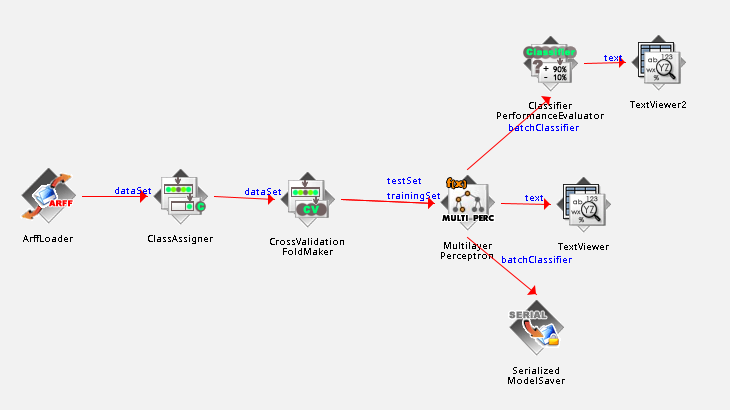
\includegraphics[scale=0.5]{img/1-seka.png}
  \caption{Užduočių seka su treniravimu ir validavimu naudojant 
  duomenų failą iris\_train\_test.arff ir kryžminę patikrą}
  \label{img:1-seka}
\end{figure}

\begin{figure}[H]
  \centering
  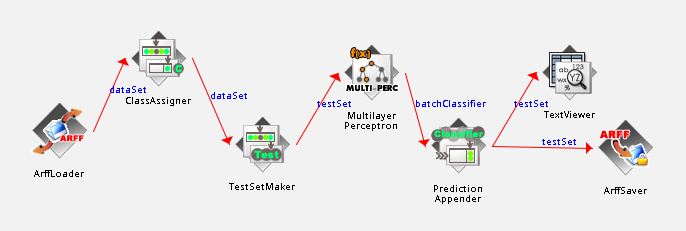
\includegraphics[scale=0.5]{img/2-seka.png}
  \caption{Užduočių seka su validavimu naudojant 
  duomenų failą iris\_new.arff}
  \label{img:2-seka}
\end{figure}

\begin{figure}[H]
  \centering
  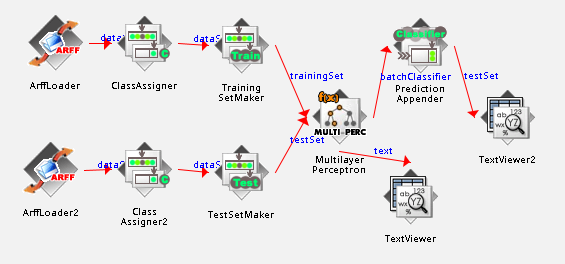
\includegraphics[scale=0.5]{img/3-seka.png}
  \caption{Užduoties seka su mokymu ir validavimu}
  \label{img:3-seka}
\end{figure}


\subsection{Pirmos užduočių sekos neuroninis tinklas}
Iš \ref{tab:parametrai} lentelės duomenų matyti, kad paslėptų
neuronų skaičius ir inercija turi labai nereikšmingą įtaką
modelio tikslumui. Taip dalinai yra todėl, kad 
duomenų rinkinys labai paprastas ir mažas, todėl užtenka
ir parpastesnio neuroninio tinklo norint pasiekti aukštą tikslumą.
Labiausiai tikslumas priklauso nuo mokymosi greičio, tą galime
matyti iš tikslumo reikšmės nukritimo nuo 96,67 \% iki 66,67 \%,
kai mokymosi greitis pakeičiamas iš 0,05 į 0,001. 

\ref{tab:parametrai} lentelės pirmos eilutės parametrai
buvo naudojami užkraunant neuroninio tinklo modelį antroje
užduoties sekoje. Neurinio tinklo vaizdas 
pateiktas \ref{img:tinklas} paveikslėlyje.

\begin{figure}[H]
  \centering
  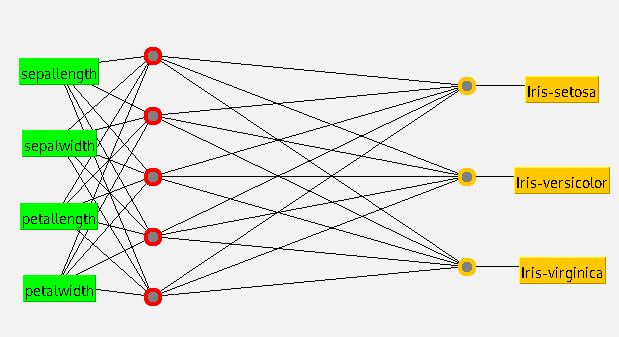
\includegraphics[scale=0.5]{img/tinklas.png}
  \caption{Neuroninio tinklo vaizdas}
  \label{img:tinklas}
\end{figure}

% Please add the following required packages to your document preamble:
% \usepackage{multirow}
\begin{table}[]
\centering
\caption{Dirbtinio neuroninio tinklo tikslumo priklausomybė nuo parametrų, epochų skaičius = 500}{
\begin{tabular}{|c|c|c|c|l}
  \cline{1-4}
  \textbf{Paslėptų neuronų sk.} & \textbf{Mokymosi greitis} & \textbf{Inercija} & \textbf{Tikslumas} &  \\ \cline{1-4}
  5                             & 0,050                     & 0,40              & 96,67 \%           &  \\ \cline{1-4}
  1                             & 0,050                     & 0,40              & 95,00 \%           &  \\ \cline{1-4}
  0                             & 0,050                     & 0,40              & 94,17 \%           &  \\ \cline{1-4}
  5                             & 0,200                     & 0,40              & 95,83\%            &  \\ \cline{1-4}
  5                             & 0,001                     & 0,40              & 66,67 \%           &  \\ \cline{1-4}
  5                             & 0,050                     & 0,10              & 96,67 \%           &  \\ \cline{1-4}
  5                             & 0,050                     & 0,80              & 96,67 \%           &  \\ \cline{1-4}
  5                             & 0,050                     & 0,01              & 95,83\%            &  \\ \cline{1-4}
  5                             & 0,050                     & 0,99              & 95,83\%            &  \\ \cline{1-4}
\end{tabular}}
\label{tab:parametrai}
\end{table}


\subsection{Klasifikavimo rezultatai iš WEKA sistemos}
Antrojoje sekoje naudjant pirmos sekos neuroninio tinklo modelį
su nauju rinkiniu (\textit{iris\_new.arff}) visos klasifikavimo
prognozės sutampa su trokštomomis klasėmis,
išskyrus vieną atvejį, kuris paršykintas \ref{tab:rezultai-2}
lentelėje. Todėl galima teigti, kad tinklas klasifikavo 
labai gerai nematytą duomenų rinkinį, kadangi tikslumas
$\frac{29}{30} * 100 \% \approx  96,67 \%$ sutampa
su mokymosi geriausiu mokymosi ir testavimo tikslumu,
kuris pateiktas \ref{tab:parametrai} lentelėje.
Taip pat iš \ref{img:scatter} pav. matyti, kad
kiekvienos klasės požymiai klasterizuojasi su
toje pačioje klasėje.


% Please add the following required packages to your document preamble:
% \usepackage[table,xcdraw]{xcolor}
% If you use beamer only pass "xcolor=table" option, i.e. \documentclass[xcolor=table]{beamer}
\begin{table}[]
  \centering
  \caption{Antros užduočių sekos prognozės naujam rinkiniui}{
  \begin{tabular}{|c|c|c|c|c|c|}
  \hline
  \textbf{sepallength} & \textbf{sepalwidth} & \textbf{petallength} & \textbf{petalwidth} & \textbf{Trokštama klasė}              & \textbf{Prognozė}                      \\ \hline
  5,1                  & 3,5                 & 1,4                  & 0,2                 & Iris-setosa                           & Iris-setosa                            \\ \hline
  4,9                  & 3                   & 1,4                  & 0,2                 & Iris-setosa                           & Iris-setosa                            \\ \hline
  4,7                  & 3,2                 & 1,3                  & 0,2                 & Iris-setosa                           & Iris-setosa                            \\ \hline
  4,6                  & 3,1                 & 1,5                  & 0,2                 & Iris-setosa                           & Iris-setosa                            \\ \hline
  5                    & 3,6                 & 1,4                  & 0,2                 & Iris-setosa                           & Iris-setosa                            \\ \hline
  5,4                  & 3,9                 & 1,7                  & 0,4                 & Iris-setosa                           & Iris-setosa                            \\ \hline
  4,6                  & 3,4                 & 1,4                  & 0,3                 & Iris-setosa                           & Iris-setosa                            \\ \hline
  5                    & 3,4                 & 1,5                  & 0,2                 & Iris-setosa                           & Iris-setosa                            \\ \hline
  4,4                  & 2,9                 & 1,4                  & 0,2                 & Iris-setosa                           & Iris-setosa                            \\ \hline
  4,9                  & 3,1                 & 1,5                  & 0,1                 & Iris-setosa                           & Iris-setosa                            \\ \hline
  7                    & 3,2                 & 4,7                  & 1,4                 & Iris-versicolor                       & Iris-versicolor                        \\ \hline
  6,4                  & 3,2                 & 4,5                  & 1,5                 & Iris-versicolor                       & Iris-versicolor                        \\ \hline
  6,9                  & 3,1                 & 4,9                  & 1,5                 & Iris-versicolor                       & Iris-versicolor                        \\ \hline
  5,5                  & 2,3                 & 4                    & 1,3                 & Iris-versicolor                       & Iris-versicolor                        \\ \hline
  6,5                  & 2,8                 & 4,6                  & 1,5                 & Iris-versicolor                       & Iris-versicolor                        \\ \hline
  5,7                  & 2,8                 & 4,5                  & 1,3                 & Iris-versicolor                       & Iris-versicolor                        \\ \hline
  6,3                  & 3,3                 & 4,7                  & 1,6                 & Iris-versicolor                       & Iris-versicolor                        \\ \hline
  4,9                  & 2,4                 & 3,3                  & 1                   & Iris-versicolor                       & Iris-versicolor                        \\ \hline
  6,6                  & 2,9                 & 4,6                  & 1,3                 & Iris-versicolor                       & Iris-versicolor                        \\ \hline
  5,2                  & 2,7                 & 3,9                  & 1,4                 & Iris-versicolor                       & Iris-versicolor                        \\ \hline
  6,3                  & 3,3                 & 6                    & 2,5                 & Iris-virginica                        & Iris-virginica                         \\ \hline
  5,8                  & 2,7                 & 5,1                  & 1,9                 & Iris-virginica                        & Iris-virginica                         \\ \hline
  7,1                  & 3                   & 5,9                  & 2,1                 & Iris-virginica                        & Iris-virginica                         \\ \hline
  6,3                  & 2,9                 & 5,6                  & 1,8                 & Iris-virginica                        & Iris-virginica                         \\ \hline
  6,5                  & 3                   & 5,8                  & 2,2                 & Iris-virginica                        & Iris-virginica                         \\ \hline
  7,6                  & 3                   & 6,6                  & 2,1                 & Iris-virginica                        & Iris-virginica                         \\ \hline
  4,9                  & 2,5                 & 4,5                  & 1,7                 & \textbf{Iris-virginica}               & \textbf{Iris-versicolor}               \\ \hline
  7,3                  & 2,9                 & 6,3                  & 1,8                 & Iris-virginica                        & Iris-virginica                         \\ \hline
  6,7                  & 2,5                 & 5,8                  & 1,8                 & Iris-virginica                        & Iris-virginica                         \\ \hline
  7,2                  & 3,6                 & 6,1                  & 2,5                 & Iris-virginica                        & Iris-virginica                         \\ \hline
  \end{tabular}}
  \label{tab:rezultai-2}
\end{table}

\begin{figure}[H]
  \centering
  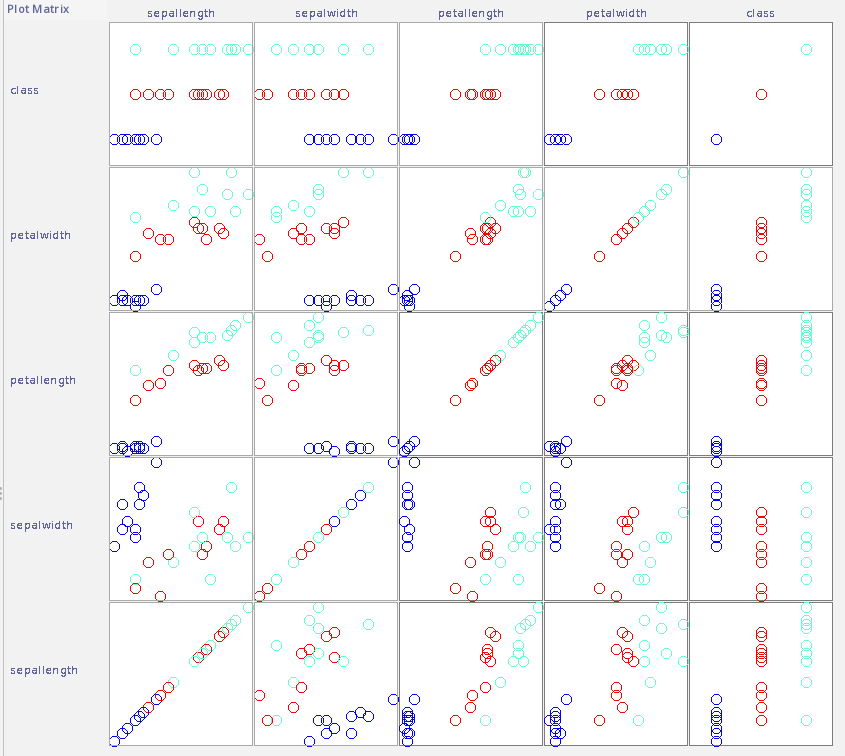
\includegraphics[scale=0.5]{img/scatter.png}
  \caption{Duomenų požymių porų vaizdai. 
  Tamsiai mėlyna — Iris-setosa, raudona — Iris-versicolor, 
  žydra — Iris-virginica}
  \label{img:scatter}
\end{figure}


\subsection{Trečios sekos modelio parametrais klasifikavimas skaičiuoklėje}
Naudojant atviro kodo skaičiuoklę \textit{LibreOffice Calc}
, trečioje sekoje gautus pirmo paslėpto sluoksnio neuronų
svorius (žr. \ref{tab:svoriai-pasleptas} lentelę) 
ir išeities trijų neuronų
svorius {žr. \ref{tab:svoriai-nepasleptas} lentelę} 
buvo sukurtas prognozavimas
skaičiuoklėje. Skaičiuoklės failą galima rasti repozitorijoje.

Neuroninis tinklas (tik klasifikavimo prognozei)
konstruojamas buvo taip: kiekvieno įrašo požymiai
buvo padauginami iš atitinkamų paslėpto tinklo neurono svorių,
kur daugybos rezultatai buvo sudedami ir dar pridedamas poslinkis.
Gauta reikšmė buvo įstatoma į sigmoidinę aktyvacijos funkciją.
Analogiška procedūra kartota ir išoriniam sluoksniui su 3 neuronais,
kur įeitys — praeitame žingsnyje gauti rezultatai po 
aktyvacijos funkcijos.

Lentėje \ref{tab:tikimybes} matyti WEKA sitemos ir
skaičiuoklės klasifikavimo tikimybės daug kur sutampa.
Nesutapimai paryškinti.
Jos sutapti visos negali, kadangi skaičiuoklė palaiko
ribotą kiekį skaičių po kablelio, dėl ko atsitinka apvalinimo
netikslimų.


\begin{table}[]
  \centering
  \caption{Paslėptojo sluoksnio svoriai. Svoriai 
    lentelėje pateikti 2 skaičių po kablelio tikslumu}{
      \begin{tabular}{|c|c|c|c|c|c|c}
        \cline{1-6}
                    & Neuronas 1 & Neuronas 2 & Neuronas 3 & Neuronas 4 & Neuronas 5 &  \\ \cline{1-6}
        poslinkis   & 2,12       & -6,10      & -5,68      & 1,81       & -1,95      &  \\ \cline{1-6}
        sepallength & 0,59       & -1,37      & -1,22      & 0,83       & -0,37      &  \\ \cline{1-6}
        sepalwidth  & -1,76      & -2,53      & -2,36      & -1,33      & 2,15       &  \\ \cline{1-6}
        petallength & 2,59       & 7,82       & 7,30       & 2,03       & -2,84      &  \\ \cline{1-6}
        petalwidth  & 2,83       & 7,78       & 7,24       & 1,68       & -3,09      &  \\ \cline{1-6}
        \end{tabular}}
  \label{tab:svoriai-pasleptas}
\end{table}


\begin{table}[]
  \centering
  \caption{Išorinio sluoksnio svoriai. Svoriai 
    lentelėje pateikti 2 skaičių po kablelio tikslumu}{
      \begin{tabular}{|c|c|c|c|c}
        \cline{1-4}
                   & Išorinis neuronas 1 & Išorinis neuronas 2 & Išorinis neuronas 3 &  \\ \cline{1-4}
        poslinkis  & 0,52                & -0,09               & -4,83               &  \\ \cline{1-4}
        Neuronas 5 & 4,93                & -5,40               & -4,93               &  \\ \cline{1-4}
        Neuronas 4 & -2,11               & 2,12                & -0,87               &  \\ \cline{1-4}
        Neuronas 3 & -1,70               & -6,45               & 6,01                &  \\ \cline{1-4}
        Neuronas 2 & -1,79               & -7,03               & 6,47                &  \\ \cline{1-4}
        Neuronas 1 & -4,25               & 3,54                & 0,76                &  \\ \cline{1-4}
        \end{tabular}}
  \label{tab:svoriai-nepasleptas}
\end{table}

\begin{table}[]
  \centering
  \caption{WEKA ir skaičiuoklės klasifikavimo prognozių tikimybės.
    Lentelėje tikimybės pateiktos 2 skaičių po kablelio tikslumu}{
        \begin{tabular}{|cc|cc|cc|l}
        \cline{1-6}
        \multicolumn{2}{|c|}{\textbf{Iris-setosa}}                       & \multicolumn{2}{c|}{\textbf{Iris-versicolor}}                   & \multicolumn{2}{c|}{\textbf{Iris-virginica}}                    &  \\ \cline{1-6}
        \multicolumn{1}{|c|}{\textbf{WEKA prog,}} & \textbf{Excel prog,} & \multicolumn{1}{c|}{\textbf{WEKA prog,}} & \textbf{Excel prog,} & \multicolumn{1}{c|}{\textbf{WEKA prog,}} & \textbf{Excel prog,} &  \\ \cline{1-6}
        \multicolumn{1}{|c|}{0,99}                & 0,99                 & \multicolumn{1}{c|}{0,01}                & 0,01                 & \multicolumn{1}{c|}{0,00}                & 0,00                 &  \\ \cline{1-6}
        \multicolumn{1}{|c|}{0,99}                & 0,99                 & \multicolumn{1}{c|}{0,01}                & 0,01                 & \multicolumn{1}{c|}{0,00}                & 0,00                 &  \\ \cline{1-6}
        \multicolumn{1}{|c|}{0,99}                & 0,99                 & \multicolumn{1}{c|}{0,01}                & 0,01                 & \multicolumn{1}{c|}{0,00}                & 0,00                 &  \\ \cline{1-6}
        \multicolumn{1}{|c|}{0,99}                & 0,99                 & \multicolumn{1}{c|}{0,01}                & 0,01                 & \multicolumn{1}{c|}{0,00}                & 0,00                 &  \\ \cline{1-6}
        \multicolumn{1}{|c|}{0,99}                & 0,99                 & \multicolumn{1}{c|}{0,01}                & 0,00                 & \multicolumn{1}{c|}{0,00}                & 0,00                 &  \\ \cline{1-6}
        \multicolumn{1}{|c|}{0,99}                & 0,99                 & \multicolumn{1}{c|}{0,01}                & 0,01                 & \multicolumn{1}{c|}{0,00}                & 0,00                 &  \\ \cline{1-6}
        \multicolumn{1}{|c|}{0,99}                & 0,99                 & \multicolumn{1}{c|}{0,01}                & 0,01                 & \multicolumn{1}{c|}{0,00}                & 0,00                 &  \\ \cline{1-6}
        \multicolumn{1}{|c|}{0,99}                & 0,99                 & \multicolumn{1}{c|}{0,01}                & 0,01                 & \multicolumn{1}{c|}{0,00}                & 0,00                 &  \\ \cline{1-6}
        \multicolumn{1}{|c|}{0,99}                & 0,99                 & \multicolumn{1}{c|}{0,01}                & 0,01                 & \multicolumn{1}{c|}{0,00}                & 0,00                 &  \\ \cline{1-6}
        \multicolumn{1}{|c|}{0,99}                & 0,99                 & \multicolumn{1}{c|}{0,01}                & 0,01                 & \multicolumn{1}{c|}{0,00}                & 0,00                 &  \\ \cline{1-6}
        \multicolumn{1}{|c|}{0,00}                & 0,00                 & \multicolumn{1}{c|}{0,99}                & 0,99                 & \multicolumn{1}{c|}{0,01}                & 0,01                 &  \\ \cline{1-6}
        \multicolumn{1}{|c|}{0,00}                & 0,00                 & \multicolumn{1}{c|}{0,99}                & 0,99                 & \multicolumn{1}{c|}{0,01}                & 0,01                 &  \\ \cline{1-6}
        \multicolumn{1}{|c|}{0,00}                & 0,00                 & \multicolumn{1}{c|}{\textbf{0,98}}       & \textbf{0,99}        & \multicolumn{1}{c|}{\textbf{0,02}}       & \textbf{0,01}        &  \\ \cline{1-6}
        \multicolumn{1}{|c|}{0,00}                & 0,00                 & \multicolumn{1}{c|}{0,99}                & 0,99                 & \multicolumn{1}{c|}{0,01}                & 0,01                 &  \\ \cline{1-6}
        \multicolumn{1}{|c|}{0,00}                & 0,00                 & \multicolumn{1}{c|}{0,98}                & 0,98                 & \multicolumn{1}{c|}{0,02}                & 0,02                 &  \\ \cline{1-6}
        \multicolumn{1}{|c|}{0,00}                & 0,00                 & \multicolumn{1}{c|}{0,99}                & 0,99                 & \multicolumn{1}{c|}{0,01}                & 0,01                 &  \\ \cline{1-6}
        \multicolumn{1}{|c|}{0,00}                & 0,00                 & \multicolumn{1}{c|}{\textbf{0,98}}       & \textbf{0,99}        & \multicolumn{1}{c|}{\textbf{0,02}}       & \textbf{0,01}        &  \\ \cline{1-6}
        \multicolumn{1}{|c|}{\textbf{0,02}}       & \textbf{0,01}        & \multicolumn{1}{c|}{0,98}                & 0,98                 & \multicolumn{1}{c|}{0,00}                & 0,00                 &  \\ \cline{1-6}
        \multicolumn{1}{|c|}{0,00}                & 0,00                 & \multicolumn{1}{c|}{0,99}                & 0,99                 & \multicolumn{1}{c|}{0,01}                & 0,01                 &  \\ \cline{1-6}
        \multicolumn{1}{|c|}{0,01}                & 0,01                 & \multicolumn{1}{c|}{0,99}                & 0,99                 & \multicolumn{1}{c|}{0,01}                & 0,01                 &  \\ \cline{1-6}
        \multicolumn{1}{|c|}{0,00}                & 0,00                 & \multicolumn{1}{c|}{0,00}                & 0,00                 & \multicolumn{1}{c|}{1,00}                & 1,00                 &  \\ \cline{1-6}
        \multicolumn{1}{|c|}{0,00}                & 0,00                 & \multicolumn{1}{c|}{0,00}                & 0,00                 & \multicolumn{1}{c|}{1,00}                & 1,00                 &  \\ \cline{1-6}
        \multicolumn{1}{|c|}{0,00}                & 0,00                 & \multicolumn{1}{c|}{0,00}                & 0,00                 & \multicolumn{1}{c|}{1,00}                & 1,00                 &  \\ \cline{1-6}
        \multicolumn{1}{|c|}{0,00}                & 0,00                 & \multicolumn{1}{c|}{0,00}                & 0,00                 & \multicolumn{1}{c|}{1,00}                & 1,00                 &  \\ \cline{1-6}
        \multicolumn{1}{|c|}{0,00}                & 0,00                 & \multicolumn{1}{c|}{0,00}                & 0,00                 & \multicolumn{1}{c|}{1,00}                & 1,00                 &  \\ \cline{1-6}
        \multicolumn{1}{|c|}{0,00}                & 0,00                 & \multicolumn{1}{c|}{0,00}                & 0,00                 & \multicolumn{1}{c|}{1,00}                & 1,00                 &  \\ \cline{1-6}
        \multicolumn{1}{|c|}{0,00}                & 0,00                 & \multicolumn{1}{c|}{\textbf{0,08}}       & \textbf{0,02}        & \multicolumn{1}{c|}{\textbf{0,92}}       & \textbf{0,98}        &  \\ \cline{1-6}
        \multicolumn{1}{|c|}{0,00}                & 0,00                 & \multicolumn{1}{c|}{0,00}                & 0,00                 & \multicolumn{1}{c|}{1,00}                & 1,00                 &  \\ \cline{1-6}
        \multicolumn{1}{|c|}{0,00}                & 0,00                 & \multicolumn{1}{c|}{0,00}                & 0,00                 & \multicolumn{1}{c|}{1,00}                & 1,00                 &  \\ \cline{1-6}
        \multicolumn{1}{|c|}{0,00}                & 0,00                 & \multicolumn{1}{c|}{0,00}                & 0,00                 & \multicolumn{1}{c|}{1,00}                & 1,00                 &  \\ \cline{1-6}
        \end{tabular}}
  \label{tab:tikimybes}
\end{table}

\section{Išvados}
Irisų duomenų rinkinys mažas ir paprastas, todėl
nemažai dalis paremtrų, kaip paslėptų neuronų skaičius,
inercija, neturi didelės įtakos neuroninio tinklo mokymui,
tačiau mokymosi greičio parametras išlieka reikšmingas. 
Geriausias modelio tikslumas gautas trečioje užduočių sekoje,
kur 120 įrašų naudojami mokymui ir likę 30 — testavimui.
Skaičiuoklėje galima atkurti modelį, galintį prognozuoti
tikimybinės klasifikavimo reikšmes su ganėtinai maža
paklaida lyginant su WEKA sistemos tais pačiais modelio parametrais.
\end{document}
